\documentclass[aps,prd,reprint,onecolumn,superscriptaddress,nofootinbib]{revtex4-2}
\usepackage{amsmath,amssymb,mathrsfs,graphicx,booktabs}
\usepackage[T1]{fontenc}
\begin{document}
\title{Finite survey windows, correlated Hubble dipoles, and attainable response discrepancies}
\author{Anonymous research draft}
\noaffiliation
\date{25 October 2026}
\begin{abstract}
A uniform bulk velocity has zero divergence, yet an angularly incomplete distance survey can mix that velocity into an apparent Hubble-rate fit. We use retained signed coefficients from four overlapping redshift windows to compare a common bulk response with a depth-independent rate dipole. Their combined fit leaves a quadratic discrepancy $T=23.3967205227$ for six residual degrees of freedom, with conditional Gaussian tail $0.00067393342$. Omitting cross-window covariance changes the same fit to $T=8.925712183$ and tail $0.177799$. We then determine which corrections can reach the unchanged 95\% reference. A depth-slope design leaves an irreducible discrepancy $15.3160$, above $12.5916$; an FP-composition proxy and a joint response reach the reference at dimensionless coefficient radii $5.7509$ and $1.5897$. Finally, a calibration-quotiented CF4 tensor has already dimensionless norm $0.0326568$, which sets a concrete target for a future physical response bound. These results specify finite-window response requirements under retained working statistics; the coefficient budgets are design sensitivities rather than measured calibration errors.
We also propagate a common Gaussian velocity field through the exact
finite-window estimator, retaining its cross-window and cross-smoothing
covariance under an explicit restricted-band model. A separate two-depth
Pantheon+ magnitude comparison retains all signed dipole and quadrupole
coordinates and gives a joint improvement of 17.2066 for 16 angular
coefficients, with conditional upper-tail probability 0.37235 under the
released selected-covariance Gaussian law.

\end{abstract}
\maketitle


\section{Motion, expansion and the survey window}
Directional distance--redshift coefficients connect kinematics to observations only through a specified observer and source congruence \cite{heinesen,maartens}. Survey depth and smoothing also enter the observed coefficients \cite{adamek}. This distinction matters when comparing an apparent Hubble dipole with a bulk-flow explanation \cite{boubel}. We carry the actual finite-window response into that comparison.

At an event, take an orthonormal material rest frame, proper separation $r n$, and the local affine velocity field
\begin{equation}
 v(rn)=b+r(HI+S+\Omega)n+O(r^2),\quad S^T=S,\quad {\rm tr}S=0,\quad\Omega^T=-\Omega.
\end{equation}
The radial channel is $v_r=b\cdot n+r[H+S:nn]+O(r^2)$: antisymmetry removes $\Omega$. Here $b$ has velocity units; $H,S,\Omega$ have rate units. A constant $b$ has $\nabla\cdot b=0$. Its speed alone cannot determine a volume-expansion shift.

For a weighted through-origin slope, direct substitution of $v_p=b+r[(\vartheta/3)I+S]n$ gives
\begin{align}
 \delta\widehat H&=b\cdot m_W+\vartheta/3+S:Q_W,\\
 m_W&=\frac{\sum_iw_ir_in_i}{\sum_iw_ir_i^2},\qquad
 Q_W=\frac{\sum_iw_ir_i^2n_in_i^T}{\sum_iw_ir_i^2}.
 \label{eq:window}
\end{align}
The inverse-length vector $m_W$ describes bulk leakage and the dimensionless tensor $Q_W$ describes angular sampling. An isotropic window has $m_W=0$ and $Q_W=I/3$, so trace-free shear also cancels from this monopole. Real windows need neither cancellation. In the joint monopole--dipole--STF fit used below, the saved response matrix performs the corresponding estimator-specific calculation rather than substituting a central distance for the window.

With signature $(-+++)$, observer-to-source $n$, acceleration $A$, and proper time, the same-congruence local optical coefficient is
\begin{equation}
 \mathcal H_u(n)=H-A\cdot n/c+\sigma:nn,\qquad d_L=cz/\mathcal H_u(n)+O(z^2).
\end{equation}
Its acceleration dipole differs from a finite-distance translation $b/r$. Assigning either interpretation to an apparent catalogue coefficient therefore requires the frame, depth response and finite-redshift remainder. The retained Cartesian axes below are ICRS J2000; they specify the estimator representation, rather than identifying a material rest frame.

\section{Retained carrier and physical question}

The saved four-window analysis represents each angular-rate estimator by a monopole, three Cartesian dipole coordinates, and five signed symmetric trace-free coordinates in ICRS J2000. The centers are $z_w=(0.025,0.040,0.060,0.080)$ with saved width $h=0.012$. Its full 36-by-36 joint covariance connects axes and windows, including shared groups. We extract the marginal 12-by-12 dipole covariance $C$ and window-major signed dipoles $y$; no conditioning on measured monopole or STF coordinates is performed. The complete apparent coefficient carrier and source covariance are retained in the accompanying \texttt{source\_carrier.json}, alongside the extracted $y,C$ and response matrices \cite{h03,physical}. This extraction does not replace those tensors by a scalar.

The retained estimator is a finite weighted angular-rate fit, $cz_i=d_{{\rm DM},i}[H_w+\mathbf D_w\cdot\mathbf n_i+\mathbf n_i^{\mathsf T}Q_w\mathbf n_i]$. Its coefficients are in ${\rm km\,s^{-1}\,Mpc^{-1}}$; they are not themselves physical expansion coefficients. The retained source uses 35,970 groups, assumes a diagonal row-scatter working law, and leaves common calibration, peculiar-velocity and selection covariance unmeasured. The original finite-window sensitivity experiment below consumes the saved statistics; the later covariance and supernova sections consume separate retained response products. It does not refit a catalogue or infer an observer-frame or cosmographic transfer.

Let $R$ stack the saved nine-by-three bulk-velocity dipole response blocks, with units ${\rm Mpc}^{-1}$, and let $G=\mathbf 1_4\otimes I_3$. The six-column baseline $X=[R,G]$ has full rank. Its model is
\begin{equation}
 y=Rb+Gd+D\eta+e,\qquad e\sim N(0,C)\quad\text{(retained working law)}.
 \label{eq:model}
\end{equation}
Here $b$ is in ${\rm km\,s^{-1}}$; $d,y,e$ are in ${\rm km\,s^{-1}\,Mpc^{-1}}$. The coefficient $\eta$ is dimensionless under our chosen $D$. The working Gaussian tail at the baseline is $6.7393\times10^{-4}$, a conditional diagnostic under the saved covariance, not survey-null coverage.

\section{Observed response fits and cross-window dependence}
\begin{table}[t]\caption{Observed finite-window response fits under the retained Gaussian working law. The last row removes only the cross-window covariance.}\label{tab:fits}\begin{ruledtabular}\begin{tabular}{lrrr}Response & $T$ & df & Conditional tail\\
bulk & 79.9870126913 & 9 & 1.62576001e-13\\
constant rate dipole & 94.5983167466 & 9 & 1.93736516e-16\\
bulk plus constant rate & 23.3967205227 & 6 & 0.00067393342\\
block diagonal & 8.9257121830 & 6 & 0.177799273\\
\end{tabular}\end{ruledtabular}\end{table}

We compare $D_w=R_wb$, $D_w=d_0$, and $D_w=R_wb+d_0$ using the actual signed dipoles and bulk-response matrices. The first two hypotheses each have three fitted coefficients; the last has six. Table~\ref{tab:fits} gives their residual discrepancies. The bulk-only fit gives $b=(-119.11,57.68,-263.59)\,{\rm km\,s^{-1}}$. The combined fit gives $b=(-272.71,118.35,-25.94)\,{\rm km\,s^{-1}}$ and $d_0=(1.4400,-0.6977,-2.4440)\,{\rm km\,s^{-1}\,Mpc^{-1}}$. The change in fitted components illustrates their dependence on the admitted response space.

The full dipole covariance is a marginal of the full 36-coordinate carrier. Fitting those 36 coordinates and profiling the remaining 24 mean coordinates freely gives the same statistic; conditioning on fixed measured monopole and STF means would use a different covariance. The accompanying independent numerical check verifies the profiling identity. The three working-law tails in Table~\ref{tab:fits} do not calibrate cosmological rarity or catalogue-wide null coverage.

Removing only cross-window blocks leaves the observed means unchanged but changes the combined tail from $0.00067393342$ to $0.177799$. Shared errors can cancel in depth differences, making those differences more precise than the individual windows. Dropping dependence removes that cancellation. Figure~\ref{fig:dipoles} shows the signed coordinates and finite-response fits; connecting the windows does not interpolate a motion history.
\begin{figure}[t]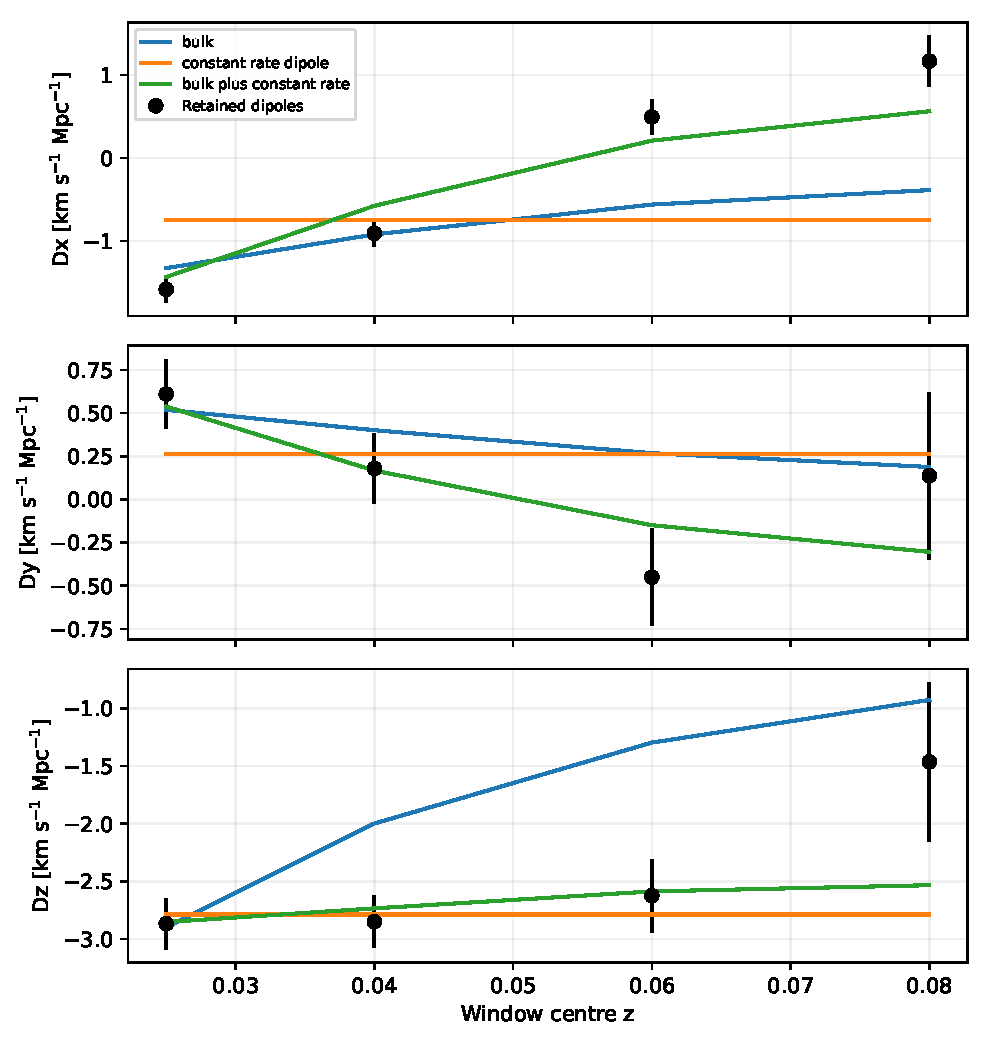
\includegraphics[width=.78\linewidth]{figures/dipole_response.pdf}\caption{Retained observed dipoles and three finite-window response fits in ICRS J2000. Error bars show marginal working standard deviations for display; every fit uses the complete cross-window covariance. The four windows overlap.}\label{fig:dipoles}\end{figure}

\section{Three fixed response mechanisms}

We specify a rate unit $u_0=1\,{\rm km\,s^{-1}\,Mpc^{-1}}$, a depth coordinate $t_w=(z_w-0.04)/h=(-1.25,0,5/3,10/3)$, and the retained FP distance-weight fractions
\begin{equation}
 p=(0.30371471,0.53491724,0.80241152,0.90188987),\qquad f_w=p_w-p_0.
\end{equation}
For window $w$ and Cartesian component $i$, each response has one coefficient per axis $a$:
\begin{equation}
 (D_z)_{(w,i),a}=u_0t_w\delta_{ia},\quad
 (D_{\rm FP})_{(w,i),a}=u_0f_w\delta_{ia},\quad
 D_{\rm joint}=[D_z,D_{\rm FP}].
 \label{eq:design}
\end{equation}
$D_z$ is a linear finite-center directional-rate slope per saved width. $D_{\rm FP}$ is a dipolar offset modulated by FP composition; subtraction of $p_0$ changes only a constant-rate column already fitted by $G$. The composition fractions do not give a signed distance-modulus calibration derivative. The joint design has six coefficients in depth-first, then FP, Cartesian order. All three are declared before seeing their residual reduction, and none is preferred as a physical error model on that basis. The common coefficient metric for each dimension is $M=I_p$: $\|\eta\|_2\leq\rho$. This is one joint sensitivity budget, not independent axis allowances or an empirical prior.

\section{Projection, ellipsoid and minimum budget}

Write $C=LL^{\mathsf T}$ without jitter, $W=L^{-1}$, $A=WX$, and let $Q_A$ have orthonormal columns spanning $A$. The orthogonal residual projector is $P=I-Q_AQ_A^{\mathsf T}$. With $r=PWy$, $B=PWD M^{-1/2}$, and $\xi=M^{1/2}\eta$, profiling the six signal coefficients reduces Eq.~(\ref{eq:model}) to
\begin{equation}
 T_{\min}(\rho)=\min_{\|\xi\|\leq\rho}\|r-B\xi\|^2,
 \quad T_0=\|r\|^2=23.3967205227. \label{eq:profile}
\end{equation}
The covariance is the complete dipole marginal; using only within-window blocks would produce $T_0=8.92571218$ and change the question. We retain the original six-degree reference $\tau=\chi^2_{6,0.95}=12.5915872437$ after minimizing over $\xi$. Replacing its degree count by $12-\operatorname{rank}[X,D]$ would create a different working-law test.

The image $\mathcal E_\rho=\{B\xi:\|\xi\|\leq\rho\}$ is generally a degenerate ellipsoid in the 12D whitened space. Cauchy--Schwarz gives its exact support in direction $u$:
\begin{equation}
 h_{\mathcal E_\rho}(u)=\rho\|B^{\mathsf T}u\|,
 \quad \xi_*=\rho\frac{B^{\mathsf T}u}{\|B^{\mathsf T}u\|}\quad(B^{\mathsf T}u\ne0).
 \label{eq:support}
\end{equation}
When $B^{\mathsf T}u=0$, support is zero and $\xi=0$ attains it. A proposed correction $q$ is attainable exactly when $q\in\operatorname{col}B$ and $\|B^+q\|\leq\rho$: the pseudoinverse is the minimum-norm preimage, while adding a kernel vector cannot lower its norm. An unrestricted 12D ball omits the column-space condition.

For the resolved thin singular-value decomposition $B=U\operatorname{diag}(\sigma_i)V^{\mathsf T}$, define $\alpha=U^{\mathsf T}r$ and $r_\perp=r-U\alpha$. The signed $r_\perp$ and all singular vectors are exported with the data. Orthogonality gives the irreducible discrepancy $T_\perp=\|r_\perp\|^2$ and saturation radius $\rho_{\rm sat}=\|\operatorname{diag}(\sigma_i^{-1})\alpha\|$. For $0<\rho<\rho_{\rm sat}$, stationarity of the convex Lagrangian $\|r-B\xi\|^2+\lambda(\|\xi\|^2-\rho^2)$ yields
\begin{align}
 \xi_\lambda&=V\operatorname{diag}\!\left(\frac{\sigma_i}{\sigma_i^2+\lambda}\right)\alpha,
 &\rho^2&=\sum_i\frac{\sigma_i^2\alpha_i^2}{(\sigma_i^2+\lambda)^2},\label{eq:kkt}\\
 T_{\min}(\rho)&=T_\perp+\sum_i\frac{\lambda^2\alpha_i^2}{(\sigma_i^2+\lambda)^2}.
 \label{eq:objective}
\end{align}
The multiplier is positive and unique on the active interval. At zero budget $T_{\min}=T_0$; at or above saturation the minimum-norm solution $B^+r$ attains $T_\perp$. If $B=0$, the discrepancy never moves. Hence the least coefficient budget for $T_{\min}\leq\tau$ is zero when $T_0\leq\tau$, unattainable when $T_\perp>\tau$, and $\rho_{\rm sat}$ when $T_\perp=\tau<T_0$. The last case is finite attainment, including equality. In the strict crossing case $T_\perp<\tau<T_0$, a unique positive multiplier solves Eq.~(\ref{eq:objective}) at $\tau$, with $\rho$ obtained from Eq.~(\ref{eq:kkt}).

For numerical classification, proximity to $\tau$ is not an exact equality identity: a computed floor within $10^{-9}$ of $\tau$ receives a boundary hold and no finite budget unless equality is established analytically. Before resolving the singular spectrum of $B$ relative to its largest value, we compare it with the positive unprojected scale $\|WD\|_{\rm op}$ for $M=I$. This prevents projection roundoff for the exact $D=X$ zero-response control from becoming apparent signal rank. The three reported designs have certified nonzero projected directions and retain the original relative-spectrum rule.

A second budget counts the image $q=\|B\xi\|$, in whitened discrepancy units. Its exact least value for the same threshold inside $\operatorname{col}B$ is
\begin{equation}
 q_{\min}=\sqrt{T_0-T_\perp}-\sqrt{\tau-T_\perp},\qquad T_\perp\leq\tau<T_0.\label{eq:qmin}
\end{equation}
This follows by moving radially toward $U\alpha$ within the image subspace. It differs from the image norm $q_{95}=\|B\xi_{95}\|$ of the least \emph{coefficient} witness. The earlier unrestricted result $\eta_{95}=\sqrt{T_0}-\sqrt\tau=1.2885530$ is an image-space comparator; $\rho$ has different units and geometry. The bound $\rho_{95}\geq\eta_{95}/\|B\|_{\rm op}$ and $q_{95}\geq\eta_{95}$ provide checks.

\section{Finite-window results}

\begin{table}[t]\caption{Conditional finite-window designs. All discrepancies use the complete 12D covariance and the unchanged six-degree working threshold. $\rho_{95}$ is a dimensionless joint coefficient budget; $q_{95}$ is its projected whitened image norm. The depth design has no finite threshold crossing.}\label{tab:budgets}\begin{ruledtabular}\begin{tabular}{lrrrrr}\text{Design}&$\operatorname{rank}B$&$T_\perp$&$\rho_{95}$&$q_{95}$&$\rho_{\rm sat}$\\
Depth slope&3&15.3160&---&---&0.7465\\
FP composition&3&6.6606&5.7509&1.7108&14.5772\\
Joint&6&0.0000&1.5897&2.7480&15.4461\\
\end{tabular}\end{ruledtabular}\end{table}

The depth response has three projected directions and leaves $T_\perp=15.3160>\tau$ even at infinite coefficient radius. The three-column FP proxy leaves $T_\perp=6.6606$ and crosses at $\rho_{95}=5.7509$, with $q_{95}=1.7108$. The six-column joint design spans all six baseline residual directions numerically, leaves a floor below $2\times10^{-28}$, and crosses at $\rho_{95}=1.5897$, with $q_{95}=2.7480$. The large $\rho_{\rm sat}$ values in Table~\ref{tab:budgets} show that crossing and complete removal are distinct events. The joint image-space minimum $q_{\min}=1.2885530$ equals the unrestricted radial comparator because the image spans the six-dimensional residual space; its minimum-coefficient witness follows a different route and has the larger $q_{95}$.

\begin{figure}[t]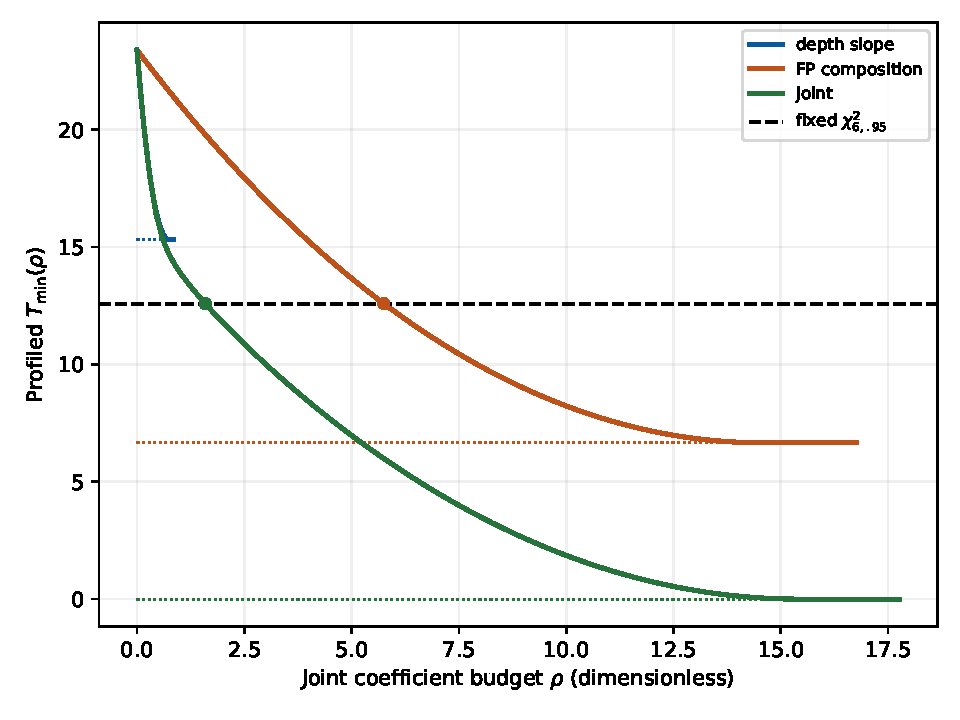
\includegraphics[width=.85\linewidth]{figures/scientific_budget.pdf}\caption{Profiled discrepancy against a \emph{joint} dimensionless coefficient radius for the three fixed finite-window designs. Dots are attained crossings of the unchanged six-degree reference; dotted horizontal lines are the irreducible floors. The depth-slope curve stays above the reference. Generated from the retained 12D covariance in ICRS J2000.}\label{fig:budget}\end{figure}
\begin{figure}[t]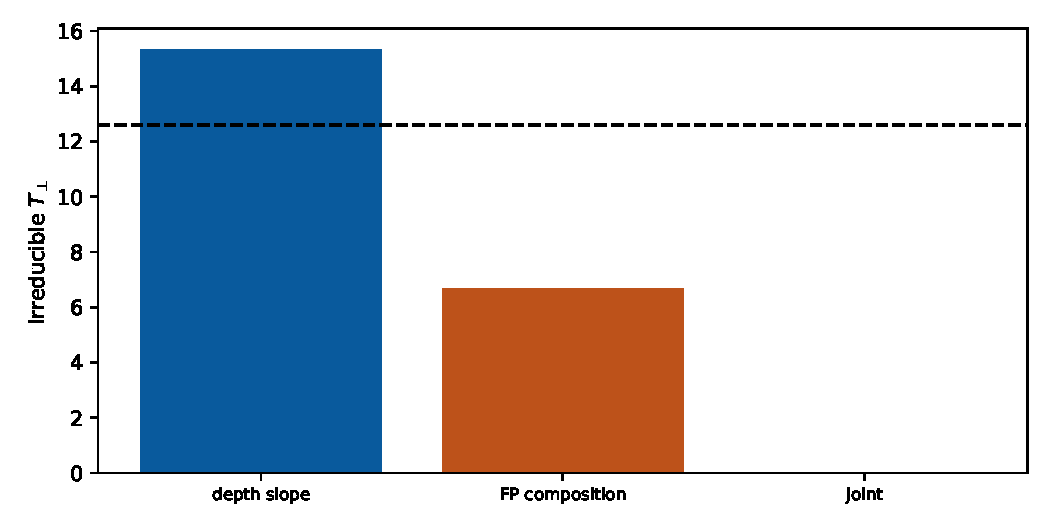
\includegraphics[width=.85\linewidth]{figures/irreducible_floor.pdf}\caption{Exact best attainable discrepancy for each declared projected response subspace. The depth-slope floor exceeds the fixed working threshold. Bars summarize the signed 12-coordinate residual vectors retained in the companion numerical product; they do not encode a physical calibration distribution.}\label{fig:floor}\end{figure}
\begin{figure}[t]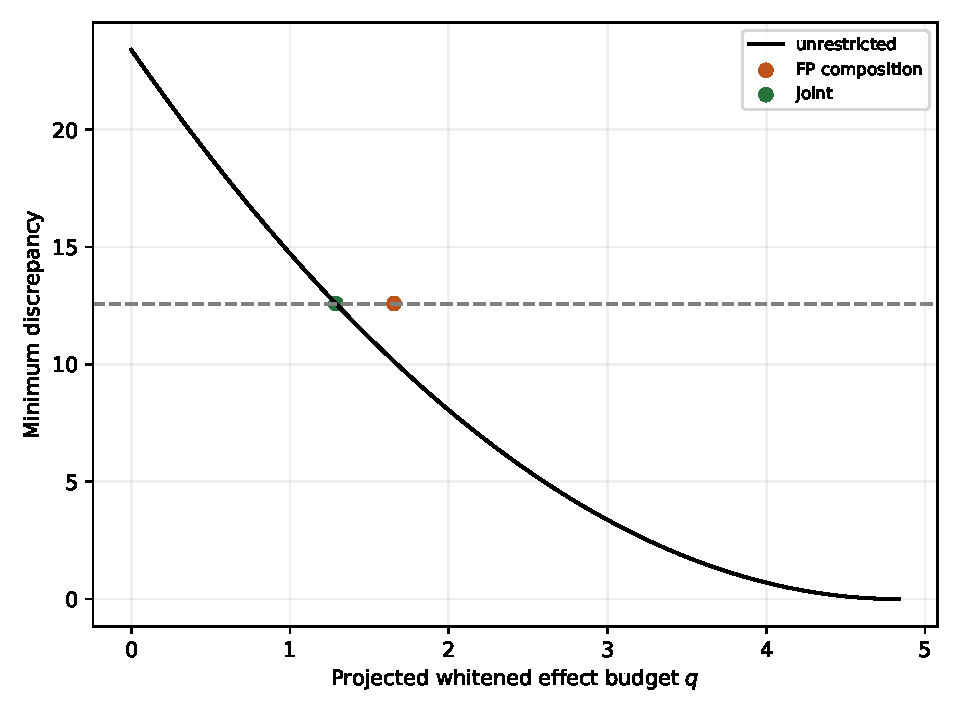
\includegraphics[width=.85\linewidth]{figures/frontier_comparison.pdf}\caption{Unrestricted 12D image-budget frontier $\max(0,\sqrt{T_0}-q)^2$ and the least image radius required by each structure. No depth-slope point exists because its irreducible floor exceeds the threshold. For the FP and joint designs, the plotted minimum-image points are distinct from the coefficient-minimizing image norms $q_{95}$ in Table~\ref{tab:budgets}.}\label{fig:frontier}\end{figure}

The computation exports the full $D$ and $B$ matrices, singular spectra, whitened residual and nonspanning remainder, threshold coefficient vectors, signed corrections, refitted $b,d$, and direct GLS residuals. The direct refits reproduce the fixed threshold within $10^{-8}$. Synthetic checks recover the wrong block-diagonal baseline, zero gain when $D=X$, nonspanning floors at arbitrarily large budgets, finite equality when the floor equals the threshold, the unrestricted radial formula when $D=L$, and invariance under a simultaneous Cartesian rotation. The computation uses the original source hashes and no source reintegration.

\section{The tensor carrier and a physical response target}
\begin{table}[t]\caption{Apparent H03 rate tensor summaries. Principal contrasts are ordered separately in each window; no common axis is tracked through depth.}\label{tab:rates}\begin{ruledtabular}\begin{tabular}{lrrrr}$z_w$ & $H_w$ & $s_1/H_w$ (\%) & $s_2/H_w$ (\%) & $s_3/H_w$ (\%)\\
0.025 & 75.1680 & -1.9917 & -0.0901 & 2.0818\\
0.040 & 75.3032 & -2.6465 & -0.5839 & 3.2304\\
0.060 & 74.5592 & -3.5464 & -0.0263 & 3.5727\\
0.080 & 72.4452 & -2.1215 & 0.5534 & 1.5681\\
\end{tabular}\end{ruledtabular}\end{table}

The signed rate tensors contain directions that a scalar contraction discards. We retain all five STF coordinates per window, their complete $3\times3$ tensors and the full joint covariance in the reproduction package. Table~\ref{tab:rates} summarizes their principal contrasts. Positive relative eigenvalues mean faster apparent expansion than the fitted mean; negative ones mean slower expansion, rather than necessarily absolute contraction. Reordering eigenvalues in each window does not follow a fixed material axis through depth.

The calibration-quotiented CF4 statistic supplies a complementary five-coordinate tensor. Its producer places $-\kappa$, with $\kappa=5/\ln10$, in the magnitude design, so it estimates a dimensionless relative-rate tensor $T$ directly. In general the conventions obey
\begin{equation}
 \delta H(n)/H=T:nn,\qquad B_\mu=-\kappa T,\qquad B_H=HT.
\end{equation}
The reference CF4 design uses the CMB-frame $V_{\rm cmb}/c$ redshift proxy, with fixed $H_0=74.6\,{\rm km\,s^{-1}\,Mpc^{-1}}$ and $\Omega_m=0.3153$. These choices do not identify a material congruence. The saved CF4 coefficient is $T$, not $B_\mu$. Applying $-\ln10/5$ again would convert it twice. The producer's orthonormal STF basis has second diagonal element $\operatorname{diag}(1,1,-2)/\sqrt6$; we decode the arrays with that sign. The complete signed tensor and eigenvalues are shown in Fig.~\ref{fig:cf4}. The Frobenius norm is $0.03265680189321492$, with principal extrema $-2.3727\%$ and $+2.2399\%$ and uniform-sphere directional rms $0.01192458$.
\begin{figure}[t]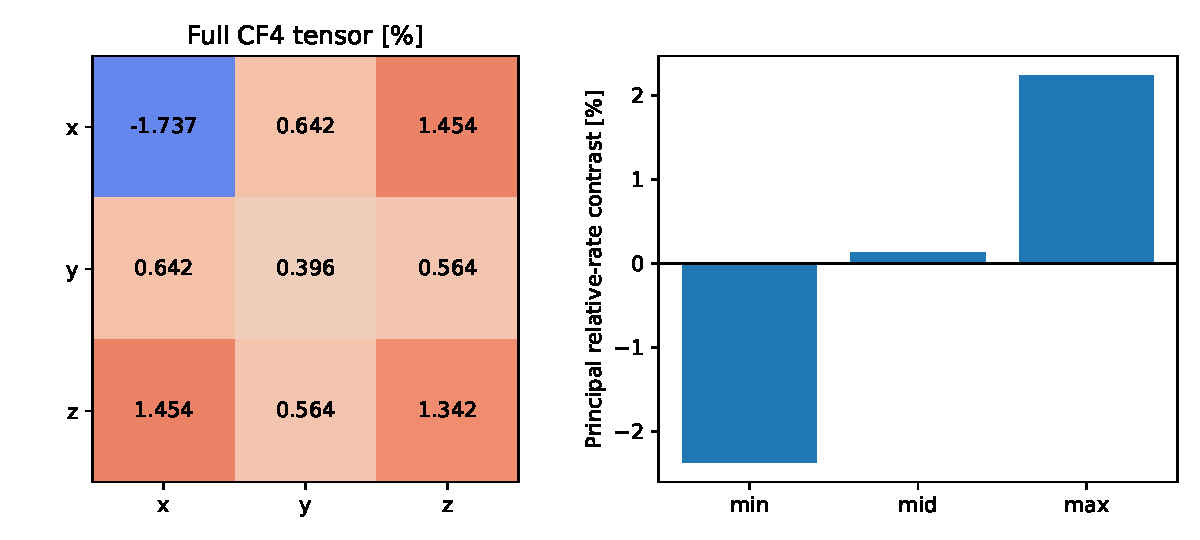
\includegraphics[width=.9\linewidth]{figures/cf4_tensor.pdf}\caption{Corrected physical reading of the retained CF4 quotient: the full dimensionless signed tensor and its ordered principal contrasts. The result uses the producer basis and no second magnitude conversion. The quotient retains five target directions numerically under its declared calibration support model; its working metric is not an empirical physical covariance.}\label{fig:cf4}\end{figure}

The finite quotient has numerical rank five under the retained tolerances and numerical annihilator residuals. The ideal support-model cancellation and its floating-point implementation remain distinct: unrestricted calibration-amplitude protection of the saved binary64 operator is not established. Peculiar-velocity, selection and physical residual covariance remain unmeasured. This defines the scope in which the displayed tensor is an apparent rate statistic.

Suppose a qualified observation response establishes $\|\widehat T-\sigma/H\|_F\leq\epsilon$ on a common event with coefficient uncertainty. The triangle inequality then gives
\begin{equation}
 \frac{(\|\widehat T\|_F-\epsilon)_+}{\sqrt6}
 \leq\Sigma\leq
 \frac{\|\widehat T\|_F+\epsilon}{\sqrt6},\qquad
 \Sigma^2=\frac{\sigma:\sigma}{6H^2}.
\end{equation}
A nonzero lower bound therefore requires a total radius below $0.0326568$. At zero radius the conditional value is $0.0133321$; this is a response-identity scenario, not a measured physical shear. A material-frame response and a justified joint error bound or law are needed to attach physical meaning or coverage. No evolution equation is supplied by the tensor contraction.

\section{Correlated velocity uncertainty through a fixed survey estimator}
A velocity-field model becomes relevant to the apparent expansion
coefficients only after it is propagated through the same estimator that
produced them. Freeze the catalogue distances, directions, weights and
row order, and write

\[
 \widehat\theta=A y,\qquad y_i=c z_{{\rm CMB},i},\qquad
 A_w=(X_w^T W_wX_w)^{-1}X_w^T W_w,
 \quad X_{w,i}=d_i(1,n_i,E_1:n_in_i,\ldots,E_5:n_in_i).
\]

The four window blocks form a 36 by 35,970 operator. The directions are
outward ICRS J2000, distances are in Mpc, the input is in km/s, and the
output coefficients are in km/s/Mpc. The released redshift defines a
fixed proxy; it is not varied as an observer parameter. The five
matrices \(E_A\) form the signed orthonormal STF basis used earlier.
Applying the same operator to a source bulk velocity and to observer
motion gives \([AN,-AN]\), where row \(i\) of \(N\) is \(n_i^T\).
Consequently \((h,h)\) is a null direction for every constant vector
\(h\). This statement concerns source minus observer velocity; the
earlier comparison between a velocity response and a constant
apparent-rate dipole is a different design comparison.

For an independent source-error component with diagonal variance \(D\),
a common velocity-field factor \(V\), and mean-design offsets \(Z\eta\)
with covariance \(\Sigma\), the propagated covariance is

\[
 C_\theta=A\operatorname{diag}(D)A^T+(AV)(AV)^T+K\Sigma K^T,
 \qquad K=AZ.
\]

Independence is part of this stipulated decomposition. Correlated source
classes require their joint factors and cross terms. The original
weighting law, \(250^2+[70(\ln10/5)d_i e_{{\rm DM},i}]^2\), already
contains a velocity-scale term and has no established empirical
decomposition. We display its propagated working covariance separately.
It is neither added to nor subtracted from the new conditional total.

The velocity calculation uses the Eisenstein--Hu no-wiggle approximation
and a common present-day Gaussian density realization, propagated with
the prescribed linear growth factors. The numerical background is
\(H_0=67.36\) km/s/Mpc, \(\Omega_m=0.3153\), \(\Omega_\Lambda=0.6847\),
\(\omega_b=0.02237\), \(n_s=0.9649\), and \(\sigma_8=0.8111\). The two
wavenumber bands are \([0.005,0.02]\) and
\([0.02,0.05]\,h\,{\rm Mpc}^{-1}\), with \(h=0.6736\). Shared Gaussian
smoothing radii are 5, 10 and 20 \(h^{-1}\) Mpc. At a positive
quadrature node, the source response is proportional to

\[
 b_i(k,\hat k)=g_i(n_i\!\cdot\!\hat k)e^{ik\hat k\cdot x_i}
 \left[\frac{P_0(k)w_k w_\Omega}{(2\pi)^3}\right]^{1/2} S_R(k),
 \qquad x_i=\chi(z_{{\rm CMB},i})n_i,
 \quad g_i=a_iH_if_iD_i.
\]

Real and imaginary projected columns give a positive-semidefinite Gram
matrix. There is no magnitude derivative in this velocity-to-rate
response. All radii and windows see the same field, yielding a full
108-coordinate covariance rather than independent blocks.

\begin{table}[htbp]
\centering\small
\caption{Propagated covariance traces in $(\mathrm{km/s/Mpc})^2$. Each band/radius row is its 36-coordinate block; inherited working covariance is separate from the stipulated total.}\label{tab:cf4cov}
\begin{tabular}{lll}
\toprule
Component & $R\;(h^{-1}\mathrm{Mpc})$ & Trace \\
\midrule
1 & 5 & 8.97773049 \\
1 & 10 & 8.85792223 \\
1 & 20 & 8.39976465 \\
2 & 5 & 8.08061983 \\
2 & 10 & 7.50105206 \\
2 & 20 & 5.65204638 \\
Combined PV & 5 & 17.05835032 \\
Inherited working & 5 & 4.76965546 \\
Stipulated total & 5 & 17.68057386 \\
\bottomrule
\end{tabular}
\end{table}

At 5 \(h^{-1}\) Mpc the two band traces sum to 17.05835032
\((\mathrm{km/s/Mpc})^2\). The original working trace is 4.76965546 in
these units. A separate total, which stipulates an independent 150 km/s
source term and four independent method mean-design offsets with
standard deviation 0.4 km/s/Mpc, has trace 17.68057386. The offsets use
\(Z_{im}=d_i1_{m(i)=m}\); this is not a magnitude-zero-point derivative.
Varying the distance calibration itself would also change distances,
design and possibly weights. Power outside the two bands, nonlinear
velocities, the empirical source-selection law and calibration/PV cross
terms are not supplied by this calculation.

\begin{figure}[htbp]
\centering
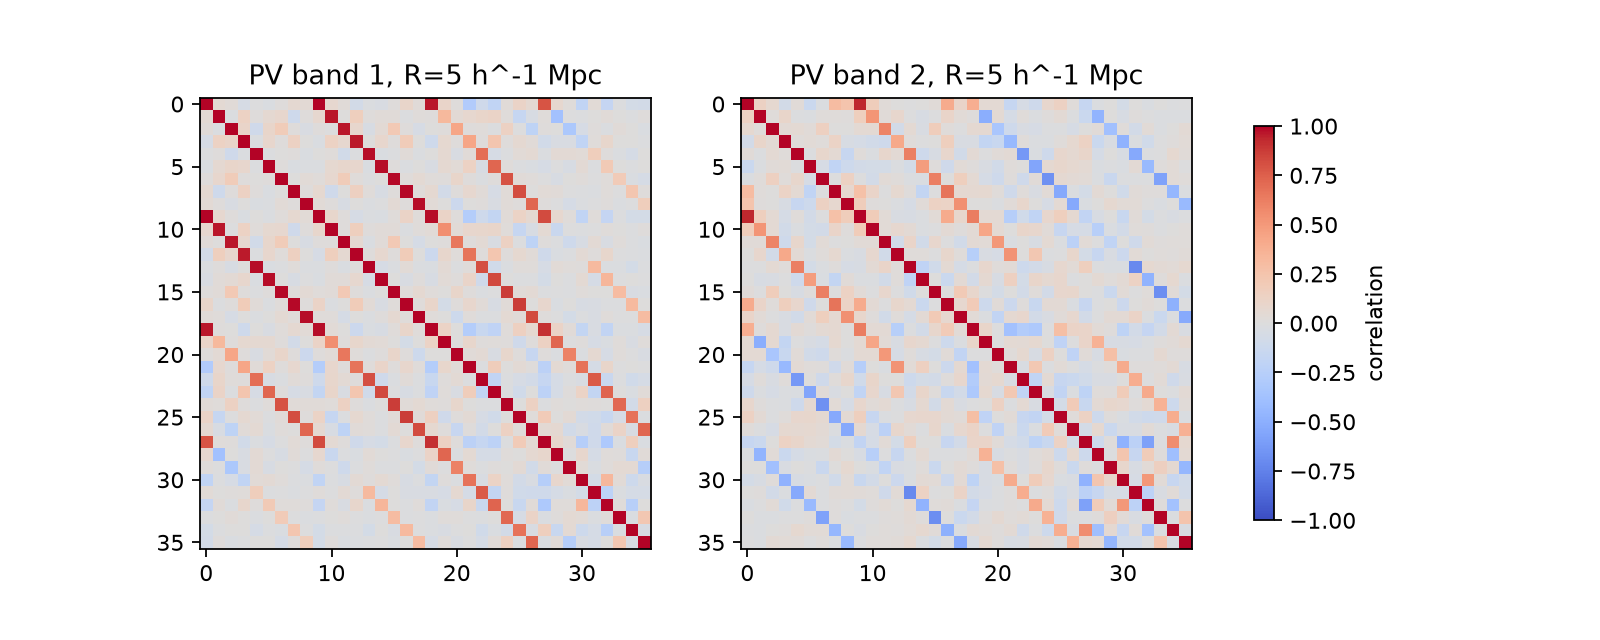
\includegraphics[width=0.95\linewidth]{r36_bridge/cf4_correlation.png}
\caption{Correlation of the propagated apparent coefficients for the two prescribed velocity bands at R=5 $h^{-1}$ Mpc. Each consecutive block of nine coordinates contains a monopole, three signed dipole components and five STF components in one redshift window. The off-diagonal blocks retain the common-source velocity field. These matrices describe the conditional Gaussian band model; they are not estimates of the complete empirical survey covariance.}
\end{figure}

\begin{table}[htbp]
\centering\small
\caption{PV trace ratios relative to the full sample at the same radius. Subsets overlap.}\label{tab:footprint}
\begin{tabular}{lllll}
\toprule
Subset & Groups & $R=5$ & $R=10$ & $R=20$ \\
\midrule
exclude\_FP & 9054 & 1.172665 & 1.172335 & 1.171046 \\
exclude\_TF & 28356 & 0.867055 & 0.866170 & 0.863461 \\
north\_ICRS\_nz\_nonnegative & 27800 & 2.404822 & 2.353335 & 2.171901 \\
south\_ICRS\_nz\_negative & 8170 & 2.580425 & 2.531798 & 2.360402 \\
\bottomrule
\end{tabular}
\end{table}

Removing or restricting catalogue subsets changes the response even
under the same field model. At the smallest radius, northern and
southern ICRS subsets have PV trace ratios 2.405 and 2.580 relative to
the full sample; removing FP or TF groups gives 1.173 and 0.867. The
corresponding ratios at the largest radius are 2.172, 2.360, 1.171 and
0.863. These are overlapping-source, footprint-dependent estimator
comparisons. They provide a quantitative reason to retain the actual
survey support, rather than independent confirmations of an anisotropic
flow.

Under the stipulated 36-coordinate total covariance at the smallest
radius, a prespecified comparison of a shared monopole, affine monopole
and shared nine-coordinate mean gives minimum discrepancies 174.925896,
145.158891 and 80.137690, with ranks 1, 2 and 9. The rule
\(T+\operatorname{rank}\ln36\) selects the nine-coordinate mean. The
retained 2,000-draw Gaussian selected-statistic reference under the
fitted shared-monopole model gives an upper-tail estimate
\(1/2001=0.00049975\), with Monte Carlo standard error approximately
0.00050. This is a finite check of that stipulated reference. It is not
an empirical CF4 population probability, and it is not directly
comparable to the earlier 12-coordinate dipole statistic, which uses a
different response and covariance. A sample-covariance inverse
correction alone would not validate a selected statistic; for example,
the Gaussian 64-mock, 36-coordinate inverse factor \(26/63\) leaves
finite-covariance uncertainty to be propagated.

\section{A released-magnitude angular comparison in two depth bins}
A second observable can be studied without assigning the apparent CF4
tensor to a matter shear. We use the released Pantheon+ corrected
magnitudes and their total statistical-plus-systematic covariance,
retaining the original observation order and repeated supernova
observations. The primary sample contains 490 noncalibrator rows with
\(0.0233\le z_{\rm HD}\le0.15\); the lower-redshift sensitivity sample
contains 705 rows with \(0.01\le z_{\rm HD}\le0.15\). Both split at
\(z_{\rm HD}=0.06\), giving 342/148 and 557/148 low/high rows
respectively. The samples overlap.

Define the fixed dimensionless reference and residual

\[
 \mu_{\rm ref}=5\log_{10}\left[(1+z_{\rm HEL})
 \int_0^{z_{\rm HD}}\frac{dz}{\sqrt{0.3153(1+z)^3+0.6847}}\right],
 \qquad y=m_{b,\rm corr}-\mu_{\rm ref}.
\]

An additive magnitude intercept and one high-bin offset are profiled.
Neither is an independent absolute-Hubble-constant measurement. In each
bin, the angular response is \(d\cdot n+\sum_{A=1}^5q_A n^TE_An\), with
coefficients in magnitudes. The axes are the released RA/DEC Cartesian
chart; its physical reference-frame binding has not been established
here. The signed STF basis is

\[
 E_1=\operatorname{diag}(1,-1,0)/\sqrt2,\quad
 E_2=\operatorname{diag}(1,1,-2)/\sqrt6,\quad
 (E_3,E_4,E_5)=(e_xe_y^T+e_ye_x^T,
 e_xe_z^T+e_ze_x^T,e_ye_z^T+e_ze_y^T)/\sqrt2.
\]

Selection uses the marginal covariance \(C_s=P_s C_{\rm STAT+SYS}P_s^T\)
once, with the same original row indices on both axes. No separate
diagonal magnitude error, PV term, jitter or rescaling is added. The
complete released 1,701-row array contains 389 unordered pairs exceeding
the fixed symmetry tolerance, with maximum asymmetry
\(3.0\times10^{-8}\,\mathrm{mag}^2\). All affected pairs lie outside the
705-row selected union. Both consumed submatrices are exactly symmetric
as stored and positive definite. This validates the consumed submatrices
without certifying or repairing the unused full array.

After Cholesky whitening, both nuisance columns are projected out and
all 16 angular directions retain full rank. Let \(T_0\) and \(T_1\) be
the profiled nuisance-only and angular-model quadratic discrepancies.
Under the fixed-design Gaussian law with known selected covariance,
\(\Delta T=T_0-T_1\) has a conditional \(\chi^2_{16}\) reference. The
nominal 95-percent threshold is 26.2962.

\begin{table}[htbp]
\centering\small
\caption{Selected released-magnitude Gaussian comparisons; the total covariance is used once.}\label{tab:snfit}
\begin{tabular}{lllllll}
\toprule
Cohort & Low/high & $T_0$ & $T_{\rm dip}$ & $T_1$ & $\Delta T$ & $p$ \\
\midrule
Primary & 342/148 & 433.458517 & 426.408712 & 416.251929 & 17.206588 & 0.372352 \\
Lower redshift & 557/148 & 608.502006 & 598.873215 & 591.947917 & 16.554089 & 0.415003 \\
\bottomrule
\end{tabular}
\end{table}

\begin{table}[htbp]
\centering\small
\caption{All signed angular coordinates in mag, ordered $(d_x,d_y,d_z,q_1,\ldots,q_5)$. Full covariance matrices accompany the numerical supplement.}\label{tab:signed}
\begin{tabular}{lllll}
\toprule
Cohort & Coordinate & Low & High & High minus low \\
\midrule
Primary & 1 & +0.017576 & +0.002231 & -0.015344 \\
Primary & 2 & +0.030016 & +0.024261 & -0.005755 \\
Primary & 3 & +0.018480 & +0.058791 & +0.040311 \\
Primary & 4 & -0.024977 & +0.007323 & +0.032300 \\
Primary & 5 & -0.003468 & +0.102639 & +0.106107 \\
Primary & 6 & -0.028210 & -0.030533 & -0.002323 \\
Primary & 7 & +0.032482 & -0.036358 & -0.068840 \\
Primary & 8 & -0.036704 & -0.057764 & -0.021059 \\
Lower redshift & 1 & +0.016817 & +0.000080 & -0.016737 \\
Lower redshift & 2 & +0.031257 & +0.022736 & -0.008520 \\
Lower redshift & 3 & +0.025519 & +0.059176 & +0.033657 \\
Lower redshift & 4 & -0.006005 & +0.011789 & +0.017794 \\
Lower redshift & 5 & +0.006537 & +0.101451 & +0.094915 \\
Lower redshift & 6 & -0.019782 & -0.026867 & -0.007086 \\
Lower redshift & 7 & +0.023529 & -0.041688 & -0.065217 \\
Lower redshift & 8 & -0.027199 & -0.059823 & -0.032624 \\
\bottomrule
\end{tabular}
\end{table}

The primary improvement is 17.206588 with conditional upper-tail
probability 0.372352; lowering the minimum redshift gives 16.554089 and
0.415003. The primary comparison does not reject its isotropic two-level
nuisance model under this conditional law. Sixteen leave-one-survey
comparisons retain angular rank 16 and give improvements from 14.0415 to
18.9251. These correlated deletions describe sensitivity; they do not
calibrate an independent population null. All 50,616 low/high covariance
entries in the primary selected matrix are nonzero, and the complete
cross-bin covariance is retained.

\begin{figure}[htbp]
\centering
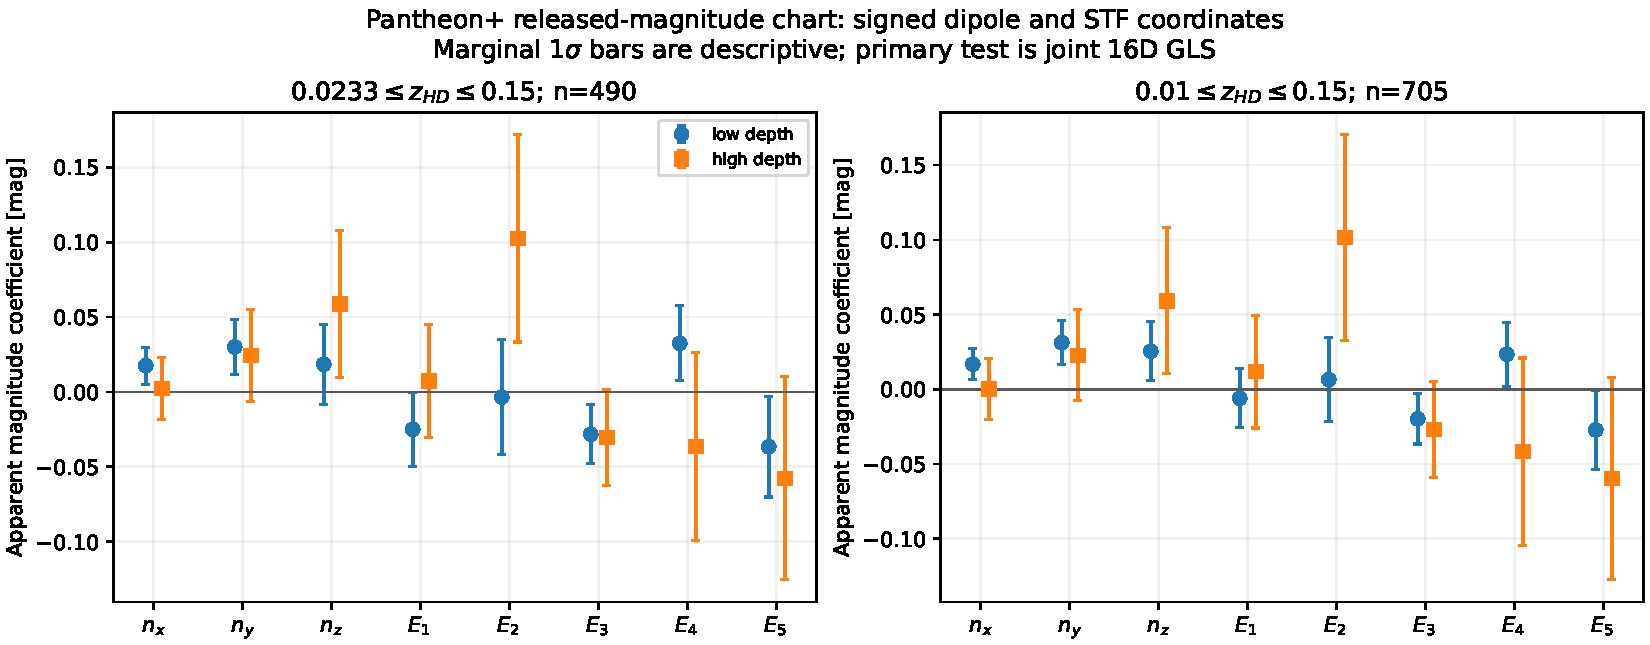
\includegraphics[width=0.95\linewidth]{r36_bridge/sn_signed.pdf}
\caption{Signed apparent-magnitude dipole and STF coordinates in the released Cartesian chart for the primary and overlapping lower-redshift sample. Error bars are marginal one-standard-deviation displays. Inference uses the full joint covariance and the prespecified 16-coordinate comparison; individual bars are not simultaneous acceptance intervals or separate binwise tests.}
\end{figure}

The chart \(d_{L*}=d_L/(1+z_{\rm HEL})^2\) subtracts
\(10\log_{10}(1+z_{\rm HEL})\) from both observed magnitude and
reference mean at fixed released redshifts. The residual and its fitted
coefficients are therefore invariant; the retained real-data coefficient
change is below \(10^{-14}\) mag. Subtracting from only one side changes
the residual and fails this consistency test. A physical observer boost
also changes photon redshift, direction, distance response and
potentially selection and uncertainty, so chart invariance is not a
boosted-observer fit. The released \(z_{\rm HD}\) includes its
peculiar-velocity correction; \(z_{\rm CMB}\) is retained and is not
substituted for the photon-redshift factor.

These magnitude tensors are a separate released-observable estimand.
They do not establish nominal light-curve-training parity, a
material-frame shear, acceleration, or a physical observer velocity. The
supernova and CF4 comparisons have neither a supplied common response
nor a measured shared-PV cross-covariance, so their statistics are not
added and their probabilities are not multiplied. Their useful common
output is a signed, covariance-aware description of apparent angular
structure with explicit depth support.

\section{Interpretation and required physical input}

These results identify sensitivity of a retained finite-window fit to three explicit response spaces. The FP fractions encode sample composition, not a signed calibration Jacobian; family-deletion dipole norms cannot supply such a derivative. For an actual weighted least-squares estimator $\theta=N^{-1}b$, a physical perturbation $\gamma$ requires $\partial_\gamma\theta=N^{-1}(\partial_\gamma b-(\partial_\gamma N)\theta)$, including any changed distances, design and weights. A source-bound signed window response to named calibration, peculiar-velocity or selection parameters, together with a justified joint bound or law and shared covariance, is needed to interpret $\eta$ as a physical error. The sky, observer and cosmographic transfer, finite remainder and null coverage are likewise open for stronger claims.

The result supplies a conditional structured-response frontier. Volume filling fractions, spatial exceedance probabilities, physical vorticity and global-tilt inference require additional physical response fields and a justified sampling law; they cannot be recovered from this 12D statistic alone.

\section{Conclusions}
The actual finite-window responses distinguish a common translation from a constant apparent rate dipole under the retained covariance. Their combination leaves $T=23.3967$, whereas ignoring cross-window dependence gives $8.9257$. The discrepancy has an explicit geometric interpretation: a depth slope misses part of the residual subspace, while the composition and joint designs can reach the fixed reference at finite coefficient radii. Those radii quantify a requirement on a proposed correction. They do not measure its physical amplitude.

A physical extension can now target named signed calibration or selection responses and their joint law, or bound the response from a material velocity gradient to the apparent CF4 tensor. The retained norm gives a quantitative scale for that task. These are finite observational-response questions which can be addressed without integrating a native cosmological solver.

\appendix
The additional covariance transport demonstrates how a shared velocity
field changes the joint apparent-coefficient uncertainty through the
actual survey operator. The released-magnitude comparison gives a
distinct observational application with its own angular response and
covariance. Their physical combination requires source, observer-frame
and cross-survey error models; those requirements cannot be replaced by
treating the two apparent tensors as measurements of one material shear.

\section{Reproduction from retained statistics}
The companion \texttt{consumer.py} reads only cached sufficient statistics, checks source SHA-256 bindings, extracts the complete dipole marginal, refits the three responses and generates the tables and vector figures. It reuses the approved structured-response implementation, including exact-zero and threshold-boundary controls, with its source identity recorded in \texttt{inputs/SOURCE\_BINDINGS.json}. The package retains the full 36-coordinate source, four complete rate tensors, corrected CF4 five-coordinate carrier and its working metric, rather than replacing them with norms. The inherited source estimator used diagonal row scatter; cross-window covariance is retained at the summary level. No raw galaxy catalogue is required by this consumer. The source-bound independent checks and research derivations are included for the stated physical identities.
\bibliographystyle{apsrev4-2}
\bibliography{references}
\end{document}
